If the context of the mission is established, the property of the robots are not :
  
\begin{itemize}[label=$-$,itemsep=0cm,topsep=0cm]
\item The robots will have a maximum range of intercommunication;
\item The robots will have a maximum range of beacons detection;
\item The robots have access to their heading and speed;
\item The beacons are recognizable;
\item The beacons do not move during the mission;
\item The beacons can ping themselves and transmit the information to the robots;
\item The distance information and communication are not available continuously.
\end{itemize}

\section{SLAM} \label{sec:slamtheory}

As seen in~\ref{sec:slamIA} the SLAM with recognizable landmarks can be done (and has been done) with constraint propagation.

\subsection{One robot}

\subsubsection*{Contractors}\label{sssec:contract}
For the SLAM two contractors are needed (see ~\ref{sec:srIA}), a distance contractor between the robot and a beacon position, for the beacons between themselves (as they can know their distances), a robot state contractor to spread the constraint over the time.

\subparagraph{Distance Contractor}
The Distance contractor is based on a simple function, the euclidean distance:

\begin{equation}
(R_{x}-B_{x})^{2}+(R_{y}-B_{y})^{2} = d_{RB} 
\end{equation}

Where R is the box containing the robot and B the box for the beacon and $d_{RB}$ the interval of the measure. This contractor with the euclidean distance is not very efficient, indeed if the pose of the robot is known but the beacon has not been estimated yet, the output will be the box containing the circle with the measured distance as a rayon surrounding the robot.To improve the computation the contracted box can be cut into a grid and then the different cases would be fed to the contractor and the remaining non-empty boxes would be kept.


\begin{figure}[H]
\centering
    \begin{minipage}[b]{0.4\textwidth}
    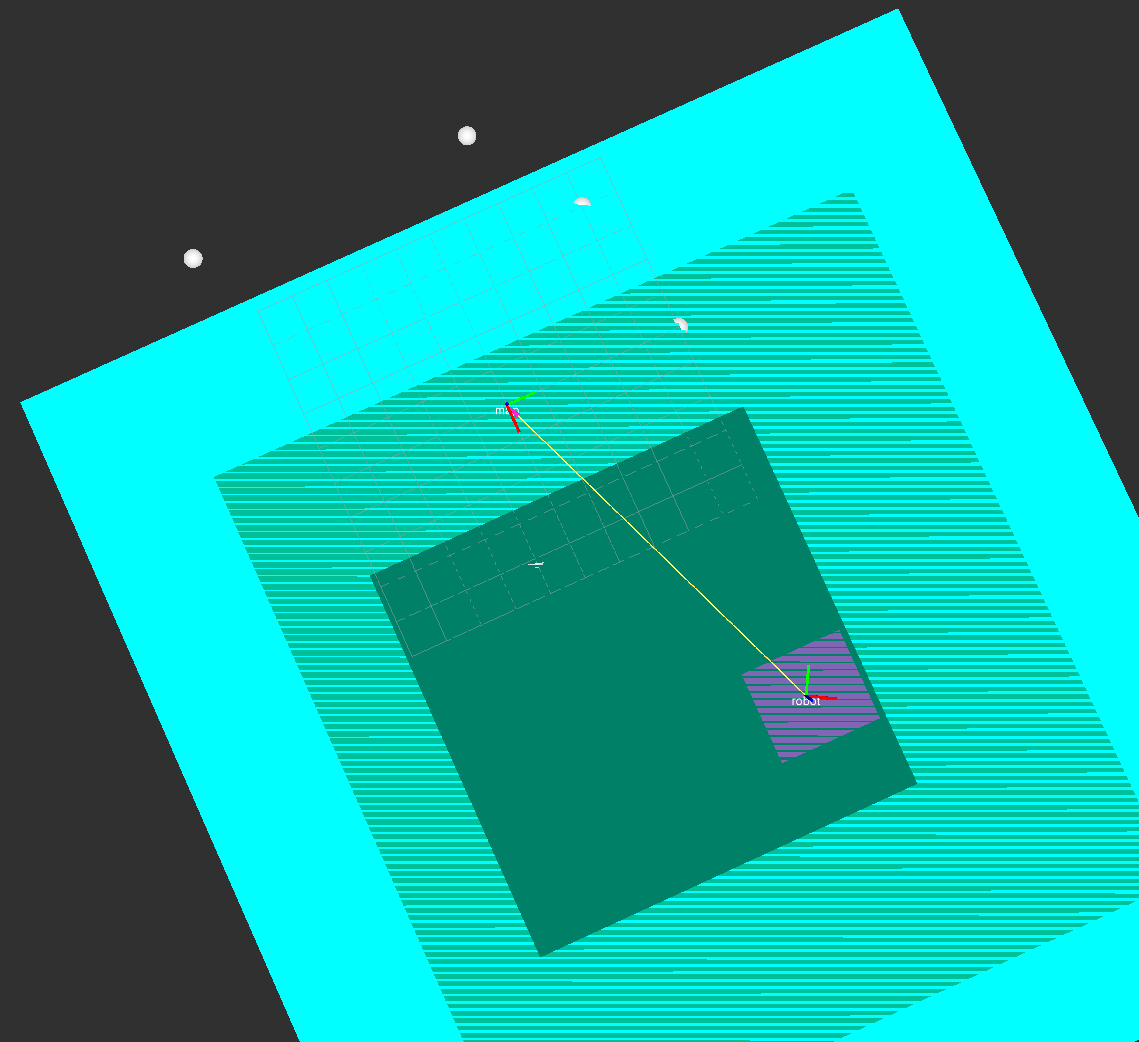
\includegraphics[scale=0.13,angle=0]{picture_no_sivia.png}
    \caption{Beacons Boxes computed without paving.}
    \label{fig:picture_no_sivia}
    \end{minipage}
    \begin{minipage}[b]{0.4\textwidth}
    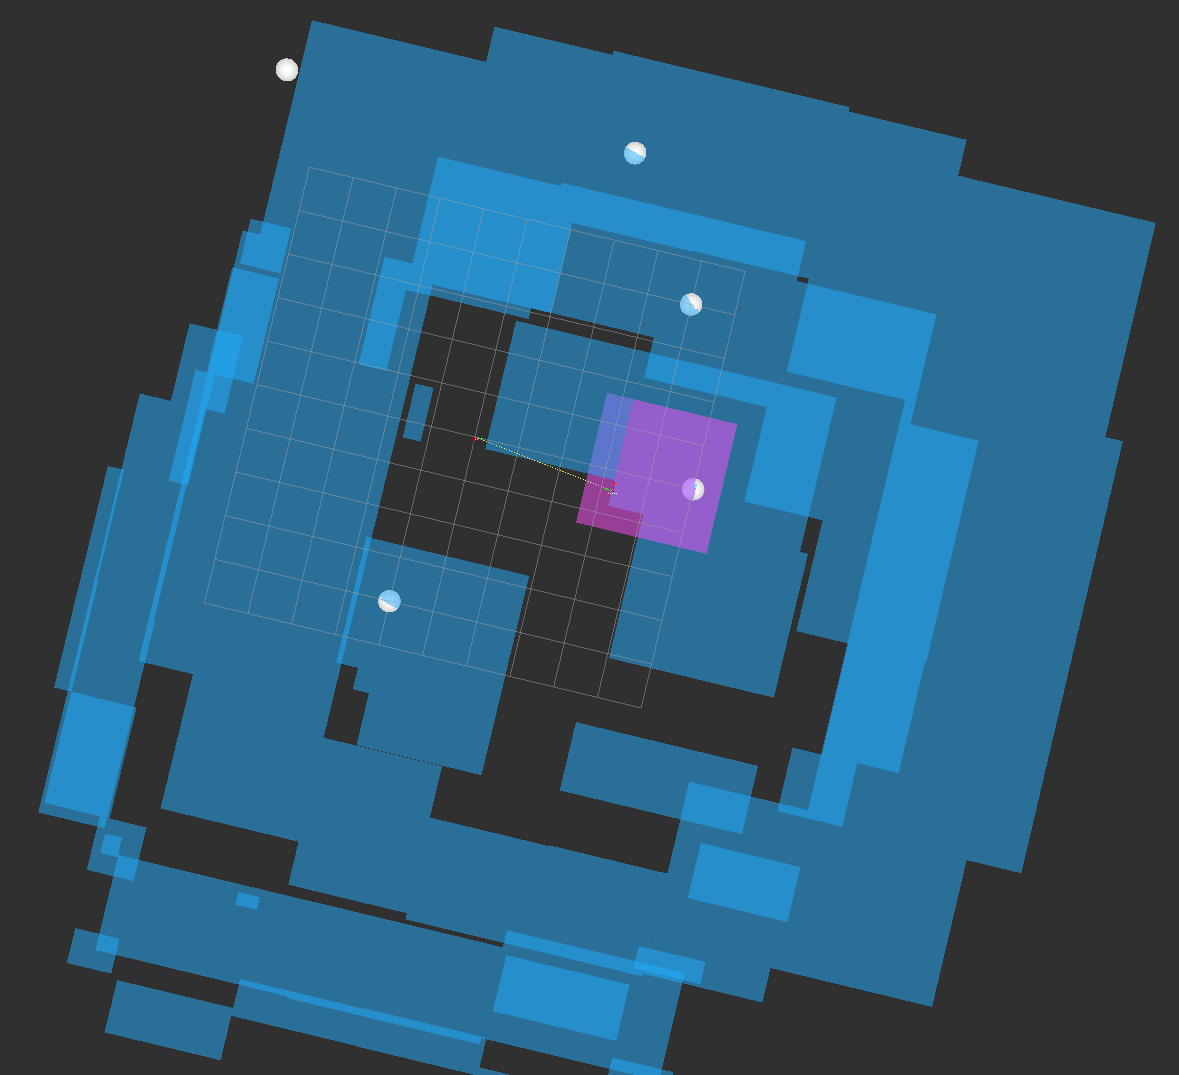
\includegraphics[scale=0.13,angle=0]{sivia_distcontraint.png}
    \caption{Beacons Box computed with paving with SIVIA \cite{jaulin1993set}.}
    \label{fig:sivia_distcontraint}
    \end{minipage}
\end{figure}

In figure~\ref{fig:picture_no_sivia} the position will be difficult to improve and in ~\ref{fig:sivia_distcontraint} the estimates of the beacons are better as the space between the robot and a beacon is not considered as a feasible position.

\subparagraph{Robot State Contractor}

 The interest of this contractor is to use a the contraction made by a beacon a a time $t_{1}$ to improve the estimate the robot over the time which can then improve the estimate of a beacon via a measure at a time $t_{2}$.

The contractor is made by knowing how the robot can move therefore the state equation of the robot is needed, for the report the state equation of a car is used:

\begin{align}
\dot{x} &= v*cos(\theta)\\
\dot{y} &= v*sin(\theta)\\
\dot{\theta} &= u_{1}\\
\dot{v} &= u_{2}
\end{align}

Then considering $u$ the input of the robot, $dt$ the incrementation duration, the time $t_{1}$ and the time $t_{2}=t_{1}+dt$ and $X(t)$ the state vector at the time $t$ the contractor is based on the following equation:  

\begin{align}
X_{0}(t_{2}) &= X_{0}(t_{1}) + X_{3}(t_{1})*\textnormal{cos}(X_{2}(t_{1}))*dt\,\\
X_{1}(t_{2}) &= X_{1}(t_{1}) + X_{3}(t_{1})*\textnormal{sin}(X_{2}(t_{1}))*dt\\
X_{2}(t_{2}) &= X_{2}(t_{1}) + u_{1}*dt\\
X_{3}(t_{2}) &= X_{3}(t_{1}) + u_{2}*dt
\end{align}

\subsubsection*{Combining the information}

The slam is supposed to be online (done in real time) this mean as for the control of a robot an estimate of
the position is needed continuously ( > 10 Hz). At each iteration the algorithm~\ref{alg:iterSlam} is processed.

\begin{algorithm}[H]
\caption{Process information for an iteration }
\label{alg:iterSlam}
\begin{algorithmic}[1]
\REQUIRE $v(t)$,$\theta(t)$,$u(t)$\\
   $X$ : (State vector from the precedent iteration)\\
   $[\,dt]\,$ :(interval containing the duration from the last iteration)\\
   $measure_{beacons}$: (set of measures between two iteration)\\
   $Past$ (vector recording of robot estimate and measure)\\
   $n$(size of Past)\\
   $distC$ : contractor of distance\\
   $robotStateC$ : contractor of robot estimate\\
   $update$: function which update the estimate of X by taking into account the proprioceptive data.\\
   $box_{beacons}$ : Set of the estimate of the beacons  
\STATE $X \leftarrow update(X,[\,dt]\,v(t),\theta(t),u(t)) $
\STATE $Past  \leftarrow Past + \{(X,[\,dt]\,,measure_{beacons})\} $
\STATE $n  \leftarrow n+1 $
\IF{$measure_{beacons} \neq  \emptyset $}
\FOR{$i=n-1;i>1;i--$}
\STATE $(X_{i},[\,dt]\,_{i},measure_{beacons,i}) \leftarrow Past(i)$
\STATE $(X_{i+1},[\,dt]\,_{i+1},measure_{beacons,i+1}) \leftarrow Past(i+1)$
\FOR{$measure_{beacon,i} \in measure_{beacons,i}$}\label{op:distB_1}
\STATE $(X_{i},box_{beacon},measure_{beacon,i}) \leftarrow distC(X_{i},box_{beacon},measure_{beacon,i})$
\ENDFOR
\STATE $(X_{i},X_{i+1},[\,dt]\,_{i+1}) \leftarrow robotStateC(X_{i},X_{i+1},[\,dt]\,_{i+1})$
\ENDFOR
\FOR{$i=0;i<n-1;i++$}
\STATE $(X_{i},[\,dt]\,_{i},measure_{beacons,i}) \leftarrow Past(i)$
\STATE $(X_{i+1},[\,dt]\,_{i+1},measure_{beacons,i+1}) \leftarrow Past(i+1)$
\FOR{$measure_{beacon,i} \in measure_{beacons,i}$}\label{op:distB_2}
\STATE $(X_{i},measure_{beacon,i}) \leftarrow distC(X_{i},measure_{beacon,i})$
\ENDFOR
\STATE $(X_{i},X_{i+1},[\,dt]\,_{i+1}) \leftarrow robotStateC(X_{i},X_{i+1},[\,dt]\,_{i+1})$
\ENDFOR
\ENDIF
\end{algorithmic}
\end{algorithm}

This algorithm does not use all the information available when using one robots (distance between beacons) and does not use a paving for the estimation of the beacons:

When receiving data from a beacon a contractor over the distance between beacon can be computed :

\begin{algorithm}[H]
\caption{Process distance between beacons }
\label{alg:distBetBeaconsSlam}
\begin{algorithmic}[1]
\REQUIRE $measure_{beacons}$: (set of measures between two iteration)\\
   $box_{beacons}$ : Set of the estimate of the beacons\\
   $Bsender$ : beacon which has transmitted the data   
\FOR{$measure_{beacon} \in measure_{beacons}$}\label{op:distB_3}
\STATE $(box_{Bsender},box_{beacon},measure_{beacon}) \leftarrow distC(box_{Bsender},box_{beacon},measure_{beacon})$
\ENDFOR
\end{algorithmic}
\end{algorithm}

But as written in ~\ref{sssec:contract} the estimate box for the beacons can be paved, that change the precedents 
algorithms when treating with a beacon estimate (\ref{op:distB_1},\ref{op:distB_2},\ref{op:distB_3}). A algorithm for the distance constraint between two set of boxes must be executed:

\begin{algorithm}[H]
\caption{Distance Constraint Application on two set of boxes }
\label{alg:distTwoSet}
\begin{algorithmic}[1]
\REQUIRE $d$: interval of the distance\\
   $\mathbb{B_{\textnormal{1}}}$ : A set of boxes\\
   $\mathbb{B_{\textnormal{2}}}$ : A second set of boxes
\STATE $\mathbb{T_{\textnormal{1}}} \leftarrow$ Vector of empty boxes of the same size of $\mathbb{B_{\textnormal{1}}}$
\STATE $\mathbb{T_{\textnormal{2}}} \leftarrow$ Vector of empty boxes of the same size of $\mathbb{B_{\textnormal{2}}}$
\FOR{$box_1 \in \mathbb{B_{\textnormal{1}}}$}
\FOR{$box_2 \in \mathbb{B_{\textnormal{2}}}$}
\STATE $(box_{1t},box_{2t},d) \leftarrow distC(box_1,box_2,d)$
\STATE $\mathbb{T_{\textnormal{1}}}(box_1) \leftarrow \mathbb{T_{\textnormal{1}}}(box_1)  \cup box_{1t}$
\STATE $\mathbb{T_{\textnormal{2}}}(box_1) \leftarrow \mathbb{T_{\textnormal{2}}}(box_2)  \cup box_{2t}$
\ENDFOR
\ENDFOR
\STATE $\mathbb{B_{\textnormal{1}}} \leftarrow \mathbb{T_{\textnormal{1}}}\setminus\{box \in \mathbb{T_{\textnormal{1}}} \mid box = \emptyset \}$
\STATE $\mathbb{B_{\textnormal{2}}} \leftarrow \mathbb{T_{\textnormal{2}}}\setminus\{box \in \mathbb{T_{\textnormal{2}}} \mid box = \emptyset \}$
\end{algorithmic}
\end{algorithm}

With the algorithms~\ref{alg:iterSlam},~\ref{alg:distBetBeaconsSlam},~\ref{alg:distTwoSet} it is possible to do a range only slam with a unique robot (see chapter~\ref{ch:results} for more details).

\subsection{With more robots}

When using multiple robots, each robot can obtain the estimations of the map from the other robots (if there is transmission), in the context of the mission the first position is known (the box for the pose estimate has a little width depending on the GPS data) therefore the position of the boxes is sure between the robots. When receiving data from another robots, one robot will fuse the estimates of the beacons from the other robots with its own estimates:

\begin{algorithm}[H]
\caption{Fusion of beacon estimate between robots}
\label{alg:fuseDataRobotSet}
\begin{algorithmic}[1]
\REQUIRE $b$: a beacon\\
   $\mathbb{B_{\textnormal{1}}}$ : set of boxes estimating the beacon b by the robot receiving the data\\
   $\mathbb{B_{\textnormal{2}}}$ : set of boxes estimating the beacon b by the robot sending the data
\STATE $\mathbb{T_{\textnormal{1}}} \leftarrow$ Vector of empty boxes of the same size of $\mathbb{B_{\textnormal{1}}}$
\FOR{$box_1 \in \mathbb{B_{\textnormal{1}}}$}
\FOR{$box_2 \in \mathbb{B_{\textnormal{2}}}$}
\STATE $\mathbb{T_{\textnormal{1}}}(box_1) \leftarrow  \mathbb{T_{\textnormal{1}}}(box_1)  \cup (box_{1} \cap box_{2})$
\ENDFOR
\ENDFOR
\STATE $\mathbb{B_{\textnormal{1}}} \leftarrow \mathbb{T_{\textnormal{1}}}\setminus\{box \in \mathbb{T_{\textnormal{1}}} \mid box = \emptyset \}$
\end{algorithmic}
\end{algorithm}

This contraction will supposedly greatly improve the estimation of the beacons as the robots do not start the mission at the same position they will see the world differently, therefore the intersection of their vision will be efficient.

\section{Controlling the robots}

The mission followed by the robots is to scan an area, with multiple robots the area can be divided between the robots (at least one robot by area).

\subsection{Path Generation}\label{ssec:pathgen}

The area is divided in a decided number of cases:

\begin{figure}[H]
\centering
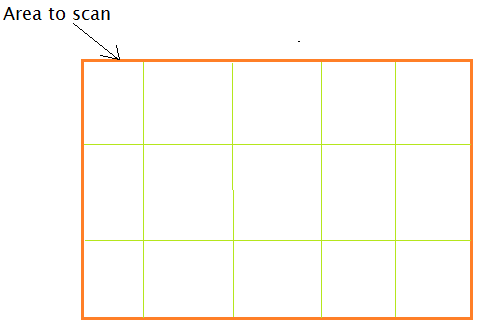
\includegraphics[scale=1]{areascanning.png}
\caption{Paving of an area to scan.}
\label{fig:areaScan}
\end{figure}

A robot will be ordered to scan a chosen case, it will make a first pass to acquire the positions of the beacons then a more thorough pass to make scan the case.

\begin{figure}[H]
\centering
    \begin{minipage}[b]{0.4\textwidth}
    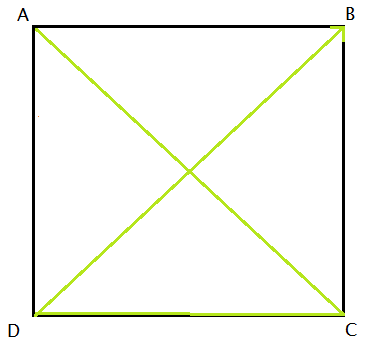
\includegraphics[scale=0.8,angle=0]{firstpass.png}
    \caption{Path of the first pass to detect beacons.}
    \label{fig:firstpass}
    \end{minipage}
    \begin{minipage}[b]{0.4\textwidth}
    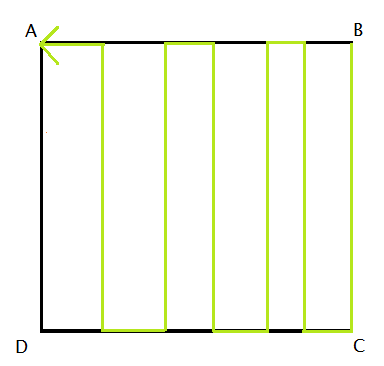
\includegraphics[scale=0.8,angle=0]{secondpass.png}
    \caption{Path of the second pass.}
    \label{fig:secondpass}
    \end{minipage}
\end{figure}

This last pass is used very often in area scanning with underwater vehicles.


\subsection{Following the path and considering the other robots}

The method chosen to control the robots for the path following and the obstacles avoidance is the potential field method. It has been chosen for its easy implementation and manipulation as itpermit to manage movable obstacles such as the other robots.
The robot is seen as an electric particle in a electric field and respond to it with the relation:

$\mathbf{f} = -\textnormal{grad}(V(\mathbf{p}))$ (page 77, ~\cite{jaulin2015mobile})\\

Where $\mathbf{p}$ is the position of the robot and $V$ its potential and $\mathbf{f}$ the force applied to the robot. If the robot need to go to a chosen point,the point will apply an attractive force on the robot and if another robot is approaching it will apply a repulsive force.

\begin{figure}[H]
\centering
    \begin{minipage}[b]{0.4\textwidth}
    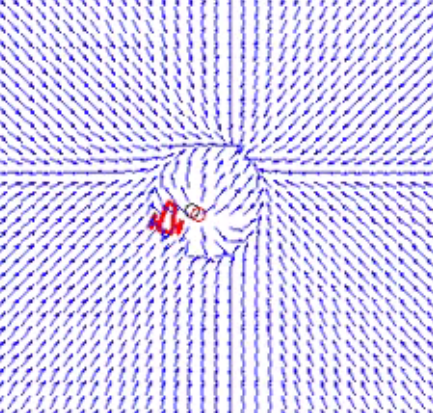
\includegraphics[scale=0.9,angle=0]{potentialCar1.png}
    \end{minipage}
    \begin{minipage}[b]{0.4\textwidth}
    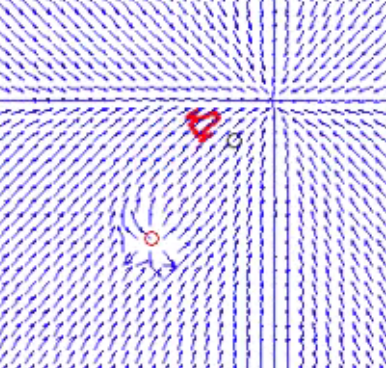
\includegraphics[scale=1,angle=0]{potentialCar2.png}
    \end{minipage}
    \caption{Car following an attractive point with potential field method with presence of a repulsive point}
    \label{fig:attractrep}
\end{figure}